% chapters/ch2-sec3b.tex -- 3.1.3 Complete Response to Impulse Input; 3.1.4 Steady State Response to Sinusoidal Forcing (PDF 149-168)
\subsubsection{Complete Response to Impulse Input}\label{ch2:sec:3.1.3}

Imagine, if you will, that the rocket considered in Section~\ref{ch2:sec:3.1.2}
encounters a step input that does \emph{not} persist for all time $t \ge 0$,
but rather ``steps down'' to zero again after some interval of time $t_1$. The
graphical representation of this forcing function, as shown in
Figure~\ref{ch2:fig:20}, forms a rectangle whose area is $M_s t_1$. Now imagine
the interval of time during which the step persists becoming shorter and
shorter as the magnitude of the applied step input becomes greater and greater
\emph{in such a way that the product $M_s t_1$, the area of the rectangle,
remains constant}. If we carry this process to its logical conclusion, we will
ultimately arrive at a configuration such that $t_1$ is zero and $M_s$ is
infinity. In this case, however, $M_s$ must be considered a rather special
``type'' of infinity, since the product of ``this'' infinity with zero has a
definite value: $M_s t_1$, which I shall hereafter denote by $H$. A forcing
function of this kind is called an \emph{impulse of strength $H$}, and the
response of a given rocket to such an input offers a second criterion by which
the resistance of the rocket to transient disturbances may be evaluated. An
impulsive input in yaw may be defined as follows:
\begin{align*}
f_x(t) &= 0 & &(t \gtrless 0)\\
f_x(t) &= \infty & &(t = 0)\\
0 \cdot f_x(t) &= H & &(t = 0)
\end{align*}
While there are more rigorous definitions of impulse inputs obtainable from
the so-called \emph{limiting arguments} of the theory of \emph{singularity
functions} (which includes, among other things, the study of steps and
impulses), such formal precision is not necessary to an understanding of the
effects of impulsive disturbances on physical systems. Like the step, the
impulse is an idealization of physical reality. You know very well that a
rocket can never encounter disturbing moments of infinite intensity and zero
duration; any \emph{strong} disturbance of \emph{short} duration, however, can
be treated as an impulse to a high order of accuracy. Momentary fluctuations in
the direction of the thrust line, oblique ejection of solid residue from the
rocket nozzle, moments arising due to launcher contact during liftoff, and
disturbances encountered during staging are examples of forcing functions
which are virtually impulsive.

\begin{figure}[htbp]
  \centering
  
\includegraphics[width=0.8\textwidth,height=0.85\textheight,keepaspectratio]{figures/ch2/fig20.png}
  \caption{Development of the concept of an impulse from a series of steps of
  finite duration. The step in (a) has an intensity $M_{s1}$ and persists for a
  time $T_1$; the product $M_{s1}T_1$ is equal to $H$ dyn-cm-sec. The step in
  (b) has an intensity $M_{s2}$ greater than $M_{s1}$, but a duration $T_2$
  less than $T_1$ such that the product $M_{s2}T_2$ is still $H$ dyn-cm-sec.
  The limiting case of this behavior is the impulse (c), a step of infinite
  intensity but infinitesimal duration such that the product of the intensity
  and the duration---called the ``strength'' of the impulse---is still $H$
  dyn-cm-sec.}
  \label{ch2:fig:20}
\end{figure}

The response to an impulsive input is conceptually somewhat more difficult to
grasp than the responses to other types of inputs. In order to facilitate a
consideration of the impulse response let me return to our discussion of the
angular acceleration of the flywheel as illustrated in Figure~\ref{ch2:fig:5}.
Recall that, for a frictionless flywheel of inertial moment $I$ to which a
constant moment $M$ is applied for a time $t$, the resulting angular velocity
of the wheel is
\begin{equation*}
\omega = \frac{Mt}{I}
\end{equation*}
and the resulting angular displacement from the original rotative position is
\begin{equation*}
\alpha = \tfrac{1}{2}\frac{M}{I}t^{2}
\end{equation*}
Suppose, now, that the moment $M$ approaches infinity and the time $t$
approaches zero in such a way that the product $Mt$ remains constant at the
value $H$. The angular velocity imparted to the wheel by the moment during the
interval $t$ will, under these conditions remain constant at the value
\begin{equation*}
\omega = \frac{H}{I}
\end{equation*}
The angular displacement $\alpha$, however, will decrease, since it is given by
\begin{equation*}
\alpha = \frac{H}{2I}t
\end{equation*}
When the limiting case is reached, the angular displacement will be zero. The
sole effect of an impulsive input to the flywheel is thus to cause a finite
angular velocity to appear instantaneously at the time of application of the
impulse.

The problem of the yawing rocket is precisely analogous, provided the damping
and corrective moments are both zero: an impulse of strength $H$ will cause an
angular velocity
\begin{equation*}
\Omega_X = \frac{H}{I_L}
\end{equation*}
to arise instantaneously, while the angular displacement at time equal to zero
will be zero. Does the presence of nonzero corrective and damping moments in
any way alter the state of the rocket at $t = 0$?

Well, it is clear that there cannot be any effect due to static stability, as
no angular displacement of the rocket has yet occurred; hence the corrective
moment at $t = 0$ is itself zero. And, although there does arise a damping
moment simultaneously with the angular velocity increment due to the impulse,
this moment is \emph{finite} and therefore can produce no change in either the
angular displacement or the angular velocity in a zero amount of time. It thus
turns out that the presence of aerodynamic moments does not modify the initial
effect upon the rocket of an impulsive input. This effect produces the
following set of initial conditions:
\begin{subequations}\label{ch2:eq:37}
\begin{equation}\label{ch2:eq:37a}
\alpha_{X0} = 0
\end{equation}
\begin{equation}\label{ch2:eq:37b}
\Omega_{X0} = \frac{H}{I_L}
\end{equation}
\end{subequations}

Unlike the step, the impulse input has associated with it no particular
response for $t > 0$. More properly speaking, the particular response is zero,
for as you can see from its definition the impulse itself is zero for all
positive values of time. A complete impulse response is actually a
\emph{homogeneous} response with a special set of initial conditions: those
given by equations~\eqref{ch2:eq:37}.

The impulse-response of an underdamped rocket is given by
equations~\eqref{ch2:eq:15} through~\eqref{ch2:eq:19}. Applying the initial
conditions given in equations~\eqref{ch2:eq:37} results in the following values
for the phase angle and the initial amplitude:
\begin{align*}
\varphi &= \arctan(0)\\
        &= 0
\end{align*}
\begin{equation*}
A = \frac{H}{I_L\omega}
\end{equation*}
The characteristic response to an impulsive disturbance is then given by
\begin{equation}\label{ch2:eq:38}
\alpha_X = \frac{H}{I_L\omega}\, e^{-Dt}\sin\omega t
\end{equation}
where $\omega$ and $D$ are determined by equations~\eqref{ch2:eq:16}
and~\eqref{ch2:eq:17}. This motion is shown in Figure~\ref{ch2:fig:21}.

\begin{figure}[htbp]
  \centering
  
\includegraphics[width=0.8\textwidth,height=0.85\textheight,keepaspectratio]{figures/ch2/fig21.png}
  \caption{Underdamped response to an impulse of strength $H$ in yaw. The
  initial angular velocity imparted by the impulse, the maximum yaw angle
  attained, and the time at which it occurs are shown.}
  \label{ch2:fig:21}
\end{figure}

The critically-damped impulse response is described by
equations~\eqref{ch2:eq:22} and~\eqref{ch2:eq:23}. In this case we have
\begin{align*}
A_1 &= 0\\
A_2 &= \frac{H}{I_L}
\end{align*}
and the characteristic motion assumes the form
\begin{equation}\label{ch2:eq:39}
\alpha_X = \frac{H}{I_L}\, t\, e^{-Dt}
\end{equation}
where $D$ is again given by equation~\eqref{ch2:eq:16}. The impulse response
of a critically-damped rocket is illustrated by Figure~\ref{ch2:fig:22}.

\begin{figure}[htbp]
  \centering
  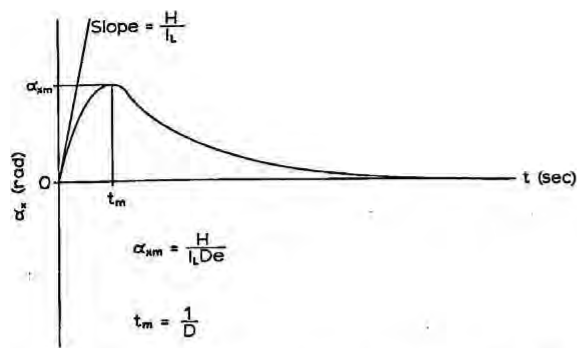
\includegraphics[width=0.8\textwidth,height=0.85\textheight,keepaspectratio]{figures/ch2/fig22.png}
  \caption{Critically damped response to an impulse of strength $H$ in yaw,
  showing the initial yaw rate, the maximum yaw angle, and the time at which
  the maximum yaw angle occurs.}
  \label{ch2:fig:22}
\end{figure}

Overdamped motion resulting from impulsive forcing obeys
equations~\eqref{ch2:eq:24} through~\eqref{ch2:eq:26}. Applying the initial
conditions to these equations gives the results
\begin{align*}
A_1 &= \frac{H\tau_1\tau_2}{I_L(\tau_1 - \tau_2)}\\
A_2 &= -\frac{H\tau_1\tau_2}{I_L(\tau_1 - \tau_2)}
\end{align*}
where $\tau_1$ and $\tau_2$ are determined by equation~\eqref{ch2:eq:25}. An
overdamped rocket will thus exhibit an impulse-response described by
\begin{equation}\label{ch2:eq:40}
\alpha_X = \frac{H\tau_1\tau_2}{I_L(\tau_1 - \tau_2)}
\left[e^{-\frac{t}{\tau_1}} - e^{-\frac{t}{\tau_2}}\right]
\end{equation}
as illustrated in Figure~\ref{ch2:fig:23}.

\begin{figure}[htbp]
  \centering
  
\includegraphics[width=0.8\textwidth,height=0.85\textheight,keepaspectratio]{figures/ch2/fig23.png}
  \caption{Overdamped response to an impulse of strength $H$ in yaw, showing
  the initial yaw rate, the maximum yaw angle, and the time at which the
  maximum yaw angle is attained. The maximum deflection occurs sooner and its
  value is smaller than is the case for the critically damped response, and
  the return to zero yaw angle is also more gradual.}
  \label{ch2:fig:23}
\end{figure}

Equation~\eqref{ch2:eq:37b} shows that the initial angular velocity resulting
from an impulsive disturbance is inversely proportional to the longitudinal
moment of inertia of the rocket which is being disturbed, and
equations~\eqref{ch2:eq:38} through~\eqref{ch2:eq:40} reveal an inverse
dependence of the initial amplitude factors on the value of $I_L$. It would
thus seem that a large $I_L$ is desirable to reduce the severity of a rocket's
impulse response. We can investigate the quantities governing the severity of
the response more thoroughly by deriving the maximum angular displacement
associated with each case of impulse-response. These maxima, and the values of
$t$ at which they occur, can be computed by setting $d\alpha_X/dt$ to zero and
determining the smallest value of $t$ that will satisfy the resulting equation.

The equation resulting from imposing the condition of zero angular velocity on
the underdamped case is
\begin{equation*}
-\frac{DH}{I_L\omega}\, e^{-Dt}\sin\omega t
+ \frac{\omega H}{I_L\omega}\, e^{-Dt}\cos\omega t = 0
\end{equation*}
from which we obtain
\begin{subequations}\label{ch2:eq:41}
\begin{equation}\label{ch2:eq:41a}
t_m = \frac{\arctan\left(\frac{\omega}{D}\right)}{\omega}
\end{equation}
so that
\begin{equation}\label{ch2:eq:41b}
\alpha_{Xm} = \frac{H}{I_L\omega}\,
e^{-\frac{D}{\omega}\arctan\left(\frac{\omega}{D}\right)}
\sin\left[\arctan\left(\frac{\omega}{D}\right)\right]
\end{equation}
\end{subequations}

For the critically-damped motion we have
\begin{equation*}
\frac{H}{I_L}\, e^{-Dt} - \frac{DH}{I_L}\, t\, e^{-Dt} = 0
\end{equation*}
from which
\begin{subequations}\label{ch2:eq:42}
\begin{equation}\label{ch2:eq:42a}
t_m = \frac{1}{D}
\end{equation}
and
\begin{equation}\label{ch2:eq:42b}
\alpha_{Xm} = \frac{H}{I_L D e}
\end{equation}
\end{subequations}

Finally, in the case of overdamped motion the applicable equation is
\begin{equation*}
-\frac{tH\tau_2}{I_L(\tau_1 - \tau_2)}\, e^{-\frac{t}{\tau_1}}
+ \frac{tH\tau_1}{I_L(\tau_1 - \tau_2)}\, e^{-\frac{t}{\tau_2}} = 0
\end{equation*}
which gives us
\begin{subequations}\label{ch2:eq:43}
\begin{equation}\label{ch2:eq:43a}
t_m = \frac{\tau_1\tau_2\ln\left(\frac{\tau_1}{\tau_2}\right)}{\tau_1 - \tau_2}
\end{equation}
where the notation ``ln'' stands for the ``natural logarithm of'' the quantity
in parentheses. Natural logarithms, also called Naperian logarithms, are the
mathematical inverse of exponential functions and may be found in tables
arranged in much the same way as are tables of trigonometric functions. From
equations~\eqref{ch2:eq:43a} and~\eqref{ch2:eq:40} we can obtain, after some
algebraic manipulation,
\begin{equation}\label{ch2:eq:43b}
\alpha_{Xm} = \frac{H\tau_1\tau_2}{I_L(\tau_1 - \tau_2)}
\left[\left(\frac{\tau_1}{\tau_2}\right)^{-\frac{\tau_2}{\tau_1 - \tau_2}}
- \left(\frac{\tau_1}{\tau_2}\right)^{-\frac{\tau_1}{\tau_1 - \tau_2}}\right]
\end{equation}
\end{subequations}

Now if you substitute the expressions derived in Section~\ref{ch2:sec:3.1.1}
for $\omega$, $D$, $\tau_1$ and $\tau_2$ into equations~\eqref{ch2:eq:41b},
\eqref{ch2:eq:42b}, and~\eqref{ch2:eq:43b} you will make the following
discoveries:
\begin{itemize}[nosep,leftmargin=2em,label={}]
  \item For underdamped motion, an increase in $I_L$ \emph{decreases}
  $\alpha_{Xm}$.
  \item For critically-damped motion, changes in $I_L$ have \emph{no effect}
  on $\alpha_{Xm}$.
  \item For overdamped motion, an increase in $I_L$ \emph{increases}
  $\alpha_{Xm}$.
\end{itemize}
These results might seem at first to indicate that large values of $I_L$ are
desirable only in the case of underdamped motion. This is not the whole story,
however, for if we examine equation~\eqref{ch2:eq:20}, in which the damping
ratio $\zeta$ is given as
\begin{equation*}
\zeta = \frac{C_2}{2\sqrt{C_1 I_L}}
\end{equation*}
we see that an increase in $I_L$ invariably \emph{reduces} the damping ratio.
In particular, increasing $I_L$ can cause overdamped or critically-damped
responses (which have already been shown to be undesirable in themselves) to
become underdamped, after which \emph{further} increases in $I_L$ will
\emph{lessen} the severity of the impulse response.

We can conclude from our analysis, then, that a large value of $I_L$ is a
desirable design characteristic in a model rocket, as a large longitudinal
moment of inertia helps both to guard against overdamping and to reduce the
rocket's sensitivity to impulsive forcing.

\subsubsection{Steady State Response to Sinusoidal Forcing}\label{ch2:sec:3.1.4}

In the previous sections we were concerned with responses to forcing functions
of a transient or discontinuous nature. The behavior of a model rocket in
these cases was such that both the homogeneous response and the particular
response were of significant importance in determining the character of the
resulting motion. In cases where the disturbing moments are of a prolonged and
periodic nature, however, the behavior of the characteristic response (which,
for positive static stability and finite damping, dies away with time) soon
creates a situation in which the particular response alone is of significant
interest. In the remainder of this section I am going to be talking about the
properties of the particular response of a rocket having a zero roll rate to
an input of the form
\begin{equation*}
f_x(t) = A_f\sin\omega_f t
\end{equation*}

The analysis will be based on the assumption that this ``sinusoidal'' input
has been going on for a time sufficiently long that all transient phenomena
have died away, so that the complete response is identical to the particular
response alone. The result obtained from an analysis based on such an
assumption is often referred to as the \emph{steady-state response to
sinusoidal forcing}, or simply the \emph{sinusoidal steady state}. Such
physical phenomena as periodic instability in the thrust line of the rocket
motor and the aerodynamic ``flutter'' of fins or control tab surfaces are
inputs which can be closely approximated by the sinusoidal representation.

Substituting the expression given above for $f_x(t)$ into
equation~\eqref{ch2:eq:13} gives us the differential equation for the yawing
oscillation in the form
\begin{equation*}
I_L\frac{d^{2}\alpha_X}{dt^{2}} + C_2\frac{d\alpha_X}{dt} + C_1\alpha_X
= A_f\sin\omega_f t
\end{equation*}
The particular solution to this equation is known to be of the form
\begin{equation}\label{ch2:eq:44}
\alpha_X = A_r\sin(\omega_f t + \varphi)
\end{equation}
The rocket responds to the sinusoidal forcing with a sinusoidal motion of its
own whose frequency is identical to the frequency of the disturbance. The
amplitude is different, however, and the response ``leads'' the forcing
function by a phase angle of $\varphi$ radians. The time derivatives of the
response thus described are
\begin{align*}
\frac{d\alpha_X}{dt} &= \omega_f A_r\cos(\omega_f t + \varphi)\\
\frac{d^{2}\alpha_X}{dt^{2}} &= -\omega_f^{2} A_r\sin(\omega_f t + \varphi)
\end{align*}
The values of $A_r$ and $\varphi$ are determined by substituting the
expressions for $\alpha_X$ and its time derivatives into the differential
equation. When this is done we obtain
\begin{align*}
&{-}I_L\omega_f^{2}A_r\sin(\omega_f t + \varphi)
+ C_2\omega_f A_r\cos(\omega_f t + \varphi) + {}\\
&\qquad C_1 A_r\sin(\omega_f t + \varphi) = A_f\sin\omega_f t
\end{align*}
It is necessary to make use of the following trigonometric identities in order
to solve this equation:
\begin{align*}
\sin(\omega_f t + \varphi) &= \sin\omega_f t\cos\varphi + \cos\omega_f t\sin\varphi\\
\cos(\omega_f t + \varphi) &= \cos\omega_f t\cos\varphi - \sin\omega_f t\sin\varphi
\end{align*}
Substitution of the quantities on the right sides of these identities for
those on the left sides in the differential equation casts it into the form
\begin{align*}
&{-}I_L\omega_f^{2}A_r\left[\sin\omega_f t\cos\varphi + \cos\omega_f t\sin\varphi\right]\\
&+ C_2\omega_f A_r\left[\cos\omega_f t\cos\varphi - \sin\omega_f t\sin\varphi\right]\\
&+ C_1 A_r\left[\sin\omega_f t\cos\varphi + \cos\omega_f t\sin\varphi\right]
= A_f\sin\omega_f t
\end{align*}
Now the terms containing $\sin\omega_f t$ and those containing
$\cos\omega_f t$ must be independent. This gives us two algebraic equations
for $A_r$ and $\varphi$:
\begin{align*}
&{-}I_L\omega_f^{2}A_r\sin\omega_f t\cos\varphi
- C_2\omega_f A_r\sin\omega_f t\sin\varphi\\
&\quad + C_1 A_r\sin\omega_f t\cos\varphi = A_f\sin\omega_f t\\[1ex]
&{-}I_L\omega_f^{2}A_r\cos\omega_f t\sin\varphi
+ C_2\omega_f A_r\cos\omega_f t\cos\varphi\\
&\quad + C_1 A_r\cos\omega_f t\sin\varphi = 0
\end{align*}
Dividing the first equation by $\sin\omega_f t$, the second by
$A_r\cos\omega_f t$ simplifies these equations to
\begin{align*}
-I_L\omega_f^{2}A_r\cos\varphi - C_2\omega_f A_r\sin\varphi + C_1 A_r\cos\varphi &= A_f\\
-I_L\omega_f^{2}\sin\varphi + C_2\omega_f\cos\varphi + C_1\sin\varphi &= 0
\end{align*}
Now the second equation can be divided by $\cos\varphi$, producing a
formulation containing the single trigonometric function $\tan\varphi$:
\begin{equation*}
\left[C_1 - I_L\omega_f^{2}\right]\tan\varphi + C_2\omega_f = 0
\end{equation*}
The phase angle is then determined as
\begin{subequations}\label{ch2:eq:45}
\begin{equation}\label{ch2:eq:45a}
\varphi = \arctan\left[\frac{C_2\omega_f}{I_L\omega_f^{2} - C_1}\right]
\end{equation}
The first equation may be divided by $\cos\varphi$ to yield
\begin{equation*}
A_r\left[\left(C_1 - I_L\omega_f^{2}\right) - C_2\omega_f\tan\varphi\right]
= \frac{A_f}{\cos\varphi}
\end{equation*}
The trigonometric identities
\begin{equation*}
\sec\varphi = \frac{1}{\cos\varphi}
\end{equation*}
and
\begin{equation*}
\sec\varphi = \sqrt{\tan^{2}\varphi + 1}
\end{equation*}
then permit us to write
\begin{equation*}
A_r\left[\left(C_1 - I_L\omega_f^{2}\right)
- \frac{C_2^{2}\omega_f^{2}}{I_L\omega_f^{2} - C_1}\right]
= A_f\sqrt{\frac{C_2^{2}\omega_f^{2}}{\left(I_L\omega_f^{2} - C_1\right)^{2}} + 1}
\end{equation*}
Some algebraic manipulation transforms this expression to
\begin{equation*}
A_r\left[\left(I_L\omega_f^{2} - C_1\right)^{2} + C_2^{2}\omega_f^{2}\right]
= A_f\sqrt{\left(I_L\omega_f^{2} - C_1\right)^{2} + C_2^{2}\omega_f^{2}}
\end{equation*}
from which we conclude that
\begin{equation}\label{ch2:eq:45b}
A_r = \frac{A_f}{\sqrt{\left(I_L\omega_f^{2} - C_1\right)^{2} + C_2^{2}\omega_f^{2}}}
\end{equation}
\end{subequations}
Now although equations~\eqref{ch2:eq:45} are perfectly acceptable solutions
for $\varphi$ and $A_r$, there is a standard formulation of these results
which greatly simplifies their interpretation. Recall from
Section~\ref{ch2:sec:3.1.1} that the natural frequency of the rocket is given
by
\begin{equation*}
\omega_n = \sqrt{\frac{C_1}{I_L}}
\end{equation*}
while the damping ratio $\zeta$ is given by equation~\eqref{ch2:eq:20}:
\begin{equation*}
\zeta = \frac{C_2}{2\sqrt{C_1 I_L}}
\end{equation*}
If we define a \emph{frequency ratio} $\beta$ as
\begin{equation}\label{ch2:eq:46}
\beta = \frac{\omega_f}{\omega_n}
\end{equation}
and an \emph{amplitude ratio} $\mathit{AR}$ as
\begin{equation}\label{ch2:eq:47}
\mathit{AR} = \frac{A_r}{A_f}
\end{equation}
we can, after some rearrangement, obtain the forms
\begin{subequations}\label{ch2:eq:48}
\begin{equation}\label{ch2:eq:48a}
\varphi = \arctan\left[\frac{2\zeta\beta}{\beta^{2} - 1}\right]
\end{equation}
\begin{equation}\label{ch2:eq:48b}
\mathit{AR} = \frac{1}{C_1\sqrt{\left(\beta^{2} - 1\right)^{2} + \left(2\zeta\beta\right)^{2}}}
\end{equation}
\end{subequations}

Graphs of the variation of phase angle and amplitude ratio with frequency
ratio for various values of $\zeta$ are given in Figures~\ref{ch2:fig:24}
and~\ref{ch2:fig:25}. In Figure~\ref{ch2:fig:24} the definition of the
arctangent function has been artificially extended to run from $\varphi = 0$
to $\varphi = -\pi$ radians so that the phase shift will appear as a
continuous function of $\beta$. Notice that for all nonzero frequencies of
disturbance the motion of the rocket \emph{lags} behind the input (that is,
$\varphi$ is negative). As $\beta$ varies from zero to infinity $\varphi$
varies from zero to $-\pi$ radians, passing through the value $(-\pi/2)$ when
$\beta = 1.0$.

\begin{figure}[htbp]
  \centering
  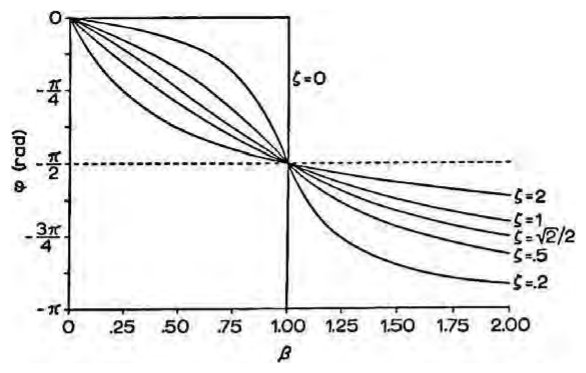
\includegraphics[width=0.8\textwidth,height=0.85\textheight,keepaspectratio]{figures/ch2/fig24.png}
  \caption{Variation of phase angle with frequency ratio for cases of
  steady-state response to sinusoidal forcing.}
  \label{ch2:fig:24}
\end{figure}

\begin{figure}[htbp]
  \centering
  
\includegraphics[width=0.8\textwidth,height=0.85\textheight,keepaspectratio]{figures/ch2/fig25.png}
  \caption{Variation of amplitude ratio with frequency ratio for cases of
  steady-state response to sinusoidal forcing. Resonant behavior can be seen
  for damping ratios less than $\sqrt{2}/2$, but does not occur at damping
  ratios greater than this value.}
  \label{ch2:fig:25}
\end{figure}

The more lightly damped the rocket, the more abrupt the transition from
$\varphi = 0$ to $\varphi = -\pi$; in the limiting case of zero damping the
transition becomes discontinuous. An examination of Figure~\ref{ch2:fig:25}
will reveal that, for rockets whose damping ratios are less than
$\sqrt{2}/2$, there exists a range of values of $\beta$ distributed about
$\beta = 1$ in which the amplitude ratio has a value greater than $1/C_1$, its
value for $\beta = 0$. This behavior is referred to as \emph{resonance}; the
greatest value of $\mathit{AR}$ attained is called the \emph{resonance peak} and the
value of $\omega_f$ at which it occurs is termed the \emph{resonant
frequency}. These quantities are computed by locating the resonance peak
analytically, using the fact that the slope of the amplitude-ratio curve is
zero there. The slope, or derivative of $\mathit{AR}$ with respect to $\beta$, is given
by the equation
\begin{equation*}
\frac{d(\mathit{AR})}{d\beta}
= \frac{-\left[\left(\beta^{2} - 1\right) + 2\zeta^{2}\right](2\beta)}
{C_1\left[\left(\beta^{2} - 1\right)^{2} + \left(2\zeta\beta\right)^{2}\right]^{3/2}}
\end{equation*}
which is zero when its numerator is zero; that is when
\begin{equation*}
\beta^{2} - 1 + 2\zeta^{2} = 0
\end{equation*}
The value of $\beta$ at resonance is therefore
\begin{subequations}\label{ch2:eq:49}
\begin{equation}\label{ch2:eq:49a}
\beta_{\mathrm{res}} = \sqrt{1 - 2\zeta^{2}}
\end{equation}
and the resonant frequency, $\omega_{\mathrm{res}}$, is given by
\begin{equation}\label{ch2:eq:49b}
\omega_{\mathrm{res}} = \beta_{\mathrm{res}}\,\omega_n
\end{equation}
\end{subequations}
By substituting $\beta_{\mathrm{res}}$ for $\beta$ in the equation for $\mathit{AR}$,
we find that the resonance peak obeys the relation
\begin{equation}\label{ch2:eq:50}
\mathit{AR}_{\mathrm{res}} = \frac{1}{2C_1\zeta\sqrt{1 - \zeta^{2}}}
\end{equation}
The value of $\mathit{AR}_{\mathrm{res}}$ can be quite large if the rocket is only
lightly damped, meaning that the amplitude of the response can be \emph{much
greater} than that of the forcing function. In fact,
equation~\eqref{ch2:eq:50} shows that the response amplitude increases
\emph{without bound} as the damping ratio decreases and becomes
\emph{infinite} at $\zeta = 0$. Resonance, therefore, can be an
\emph{extremely dangerous} state, resulting in violent oscillation of the
rocket and consequent deflection of its trajectory. The designer of model
rockets should spare no effort to minimize the effects of resonance. The use
of an adequate corrective moment coefficient (large enough static stability
margin and adequate airspeed), the maintenance of a sufficient amount of
damping, and the use of a flight velocity profile whereby the rocket passes
quickly through the resonant state due to the resulting variation in
$\omega_n$ are three techniques generally employed in various combinations for
this purpose.

As you can see from equations~\eqref{ch2:eq:49}, the resonant frequency
decreases from $\omega_n$ toward zero as the damping ratio of the rocket
increases from zero toward $\sqrt{2}/2$. This same variation in damping ratio
causes the value of the resonance peak to decrease from infinity to $1/C_1$,
and for $\zeta > \sqrt{2}/2$, there is no resonance peak at all; the value of
$\mathit{AR}$ is always less than $1/C_1$. Damping ratios greater than 0.7071
therefore result in the least severe response to disturbances of a steady
sinusoidal nature.
